\chapter{Implementierung des Prototyps}
%- Implementierung										(13 Seiten)	(13 Seiten)
Nachdem in den vergangenen Kapiteln die theoretischen Grundlagen zu Convolutional Neural Networks (CNNs) gelegt wurden, widmet sich dieses Kapitel der Implementierung des Prototyps \textit{ConvNetCPP}. Es bildet somit die Basis für das darauffolgende Kapitel, in welchem die verschiedenen Aspekte des Prototyps hinsichtlich Deep Learning experimentell untersucht werden.
Der Prototyp setzt folgende Systemparameter voraus: \\

Systemvoraussetzungen und Abhängigkeiten:
\begin{itemize}
\item Python 3.4
\item SciPy \textemdash\space Scientific Python (siehe \cite{Scipy})
\item C++11
\item Eigen-Bibliothek für Lineare Algebra  (siehe \cite{eigenweb})
\item OpenMP kompatibler Compiler (siehe  \cite{openmp08})
\item Optional: Boost Bibliotheken (siehe \cite{Schling2011})
\end{itemize}

\textit{ConvNetCPP} unterstützt insgesamt folgende Funktionen:
\begin{multicols}{2}
\begin{itemize}
\item SGD  
\item Nesterov Momentum (NAG)
\item Rprop/RMSprop
\item Equilibrium SGD
\item AdaDelta
\item L1-/L2-/Max-Norm-Penalty
\item Dropout
\item MAX-/AVG-/Stochastic-Pooling
\item Ausgabe-\textit{Padding}
\item Early Stopping
\item Sig/Tanh/ReLu
\item Softmax-Regression
\item CE/MSE-Fehlermaß
\item Conv. Denoising Autoencoder
\item Neuronen-Visualisierung
\item Ausgabe-Visualisierung 
\item Kernel-Visualisierung
\end{itemize}
\end{multicols}

\section{Architektur}
%	- Architektur (Python c++ Extension)
%		- Klassen-Diagramm
%		- Computation Pipeline
%			- Grafik OpenMP
%			- Grafik Persistency Model Matrix
%			- Grafik Model Definition File
Die Architektur von \textit{ConvNetCPP} besteht aus zwei Teilen. Den in C++ implementierten Klassen sowie einem in C geschriebenen \textit{Python Module Extension}, welches die Schnittstelle zu Python darstellt.

\subsection{C++ ConvNet}
Der C++ Teil ist aufgeteilt in 9 Klassen, welche die unterschiedlichen Teile des CNN implementieren. Die Abhängigkeiten der Klassen sind in Abbildung \ref{fig:5_class_hierarchie_autoencoder} dargestellt.

\begin{figure}
\centering
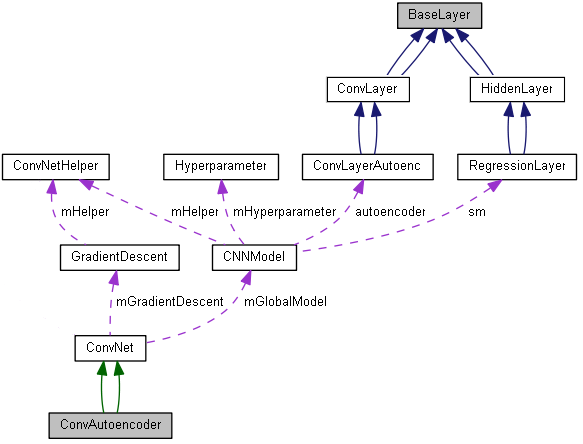
\includegraphics[width=0.8\linewidth]{images/5_class_hierarchie_autoencoder}
\caption[]{Klassenabhängigkeitsgraph des Prototyps (\textit{ConvNetCPP})}
\label{fig:5_class_hierarchie_autoencoder}
\end{figure}

Die Klasse ConvNetHelper beinhaltet die für ein CNN benötigten Basisfunktionalitäten wie das Drehen von Matrizen, Parallelisierung und die Konvertierung zwischen Vektoren und 3D-Daten für den Übergang zwischen Convolution- und Hidden-Layer. 

Optional kann die Abhängigkeit zu den Boost-Bibliotheken durch Angabe des Compiler-Flag \texttt{no\_serialization} aufgehoben werden. Damit wird die Serialisierung deaktiviert und der Status des Trainings nicht mehr länger persistiert. Dies bietet sich insbesondere unter Verwendung der Python API an, da hierbei der aktuelle Status des Models in Form einer 2D Datenstruktur an Python zurückgegeben werden.

Die vier zentralen Klassen \texttt{CNNModel}, \texttt{BaseLayer}, \texttt{ConvNet}, \texttt{ConvAutoencoder} und \texttt{Gradient\-Descent} werden im Folgenden genauer beschrieben. 

\subsubsection{CNNModel.cpp}
Die Klasse \texttt{CNNModel} repräsentiert das eigentliche CNN. Es beschreibt die Architektur und hält die Instanzen der entsprechenden Schichten des Netzwerks. 
Die Kommunikation zwischen den einzelnen Schichten geschieht mittels \textit{Messages} (vgl. Kapitel \ref{ch:cnn_back}). Diese \textit{Messages} werden durch die zwei Structs in Listing \ref{ls:struct} beschrieben. Eines definiert die Kommunikation bei der Berechnung der Netzaktivierung (\textit{Forward Pass}). Hierbei werden nur Pointer übergeben, da die entsprechenden Ausgaben pro Schicht für die Berechnungen des Gradienten weiter benötigt werden und dadurch keine Kopie der Eingabe pro Schicht erzeugt wird. Die \textit{Message} für die Rückpropagierung des Fehlers (\textit{Backward Pass}) wird nicht weiter benötigt, weshalb die Daten an die vorherige Schicht übergeben werden können.


\begin{lstlisting}[label=ls:struct,caption=Definitionen der Structs für die Kommunikation zwischen den einzelnen Schichten des CNN,captionpos=b]
struct ForwardMessage{
	vector<const vector<MatrixXd>*> vecData;
	MatrixXd* matData;
};

struct BackwardMessage{
	vector<vector<MatrixXd>> vecData;
	MatrixXd matData;
};
\end{lstlisting}

\subsubsection{BaseLayer.cpp}
Die abstrakte Klasse \texttt{BaseLayer} deklariert mehrere virtuelle Methoden, die von allen abgeleiteten Klassen implementiert werden müssen. Dies sind die für den Backpropagation-Algorithmus notwendigen Methoden für \textit{Forward Pass} und \textit{Backward Pass} sowie Methoden zur Visualisierung.
Darüber hinaus implementiert die Klasse die verschiedenen Aktivierungsfunktionen mit zugehörigen Ableitungen und Methoden zur Erzeugung gleich- oder normalverteilten Gewichten.


\subsubsection{ConvNet.cpp}
Die Klasse \texttt{ConvNet} bildet die Schnittstelle zum CNN nach außen und beinhaltet die gesamten Methoden zum Training, Prädiktion, Validierung und Visualisierung.
Die Methoden arbeiten auf Basis einer Instanz des \texttt{CNNModel}, welche außerhalb erzeugt werden muss und dem Konstruktor übergeben wird. 
Damit sind Steuerungslogik und Modelarchitektur voneinander getrennt.

\subsubsection{ConvAutoencoder.cpp}
Die Klasse \texttt{ConvAutoencoder} bildet die Schnittstelle zum Convolutional Autoencoder nach außen und beinhaltet die gesamten Methoden zum Vortraining, Prädiktion und Validierung. Die Klasse ist von \texttt{ConvNet} abgeleitet und arbeitet deshalb ebenso auf Basis einer Instanz des \texttt{CNNModel}, welche außerhalb erzeugt werden muss und dem Konstruktor übergeben wird. 

\subsubsection{GradientDescent.cpp}
Die Klasse \texttt{GradientDescent} implementiert den Gradientenabstieg und die verschiedenen Adaptionen wie Momentum und adaptive Lernraten. Da\-rüber hinaus ist in dieser Klasse auch die Max-Norm-Regularisierung implementiert, welche die Parameter unmittelbar nach einem Update auf die entsprechende Norm prüft und skaliert.
Sind die partiellen Ableitungen berechnet, wird die Instanz des \texttt{CNNModel} an \texttt{GradientDescent} übergeben und die entsprechenden Gewichtsupdates werden ausgeführt. Etwaige erweitere Algorithmen, wie das Schätzen der aktuellen Krümmung (siehe Equilibrium SGD), sind ebenfalls in dieser Klasse implementiert.


\subsection{Python Module Extension}
Python Module Extensions erlauben es in C/C++ implementierte Software in Python zur Verfügung zu stellen. Sie bilden die Standardvorgehensweise, um Python mit nativem Code zu erweitern.\footnote{Siehe dazu weitere Details in der offiziellen Python Dokumentation: \url{https://docs.python.org/3.4/extending/extending.html} (1.9.2015)}

Im Rahmen des Prototyps kann die CNN Funktionalität somit bequem durch das bereitgestellte Python Module verwendet werden, ohne auf die wichtige Performanz von nativem Code verzichten zu müssen.
Der folgende Teil beschreibt die grundlegende Konzeption der API und gibt einen Überblick der zur Verfügung stehenden Funktionen. Die Funktionen des CNN und des Convolutional Autoencoders sind aufgrund deren gemeinsamen Codebasis in einem Modul \textit{ConvNet} enthalten.

\subsubsection{Modellbeschreibung}
Im ersten Schritt wird das Modell spezifiziert. Für den Lebenszyklus eines Modells stehen die beiden Methoden \texttt{reset()} und \texttt{create()} zur Verfügung. Erstere Methode löscht bestehende Modelle, während letztere ein neues Modell erstellt.
Mehrere Modelle sind bereits vordefiniert. Spezielle Architekturen können mittels einer Konfigurationsdatei (vgl. Datei \texttt{/py\-/Model\-definition.py}) spezifiziert werden und als String der Methode \texttt{create()} übergeben werden. Dazu gehören Anzahl der Schichten, Neuronen und Zielklassen, Aktivierungsfunktionen, Dropout, Pooling, Padding sowie das Fehlermaß.

Eine weitere zur Beschreibung gehörende Methode ist \texttt{setHyperParameters()}. Diese erlaubt das Überschreiben der Standardparameter. Folgende  Hyperparameter werden bereitgestellt:

\begin{multicols}{2}
\begin{itemize}
\item INITIALIZATION
\item INIT\_STD\_DEVIATION
\item ALGORITHM
\item VISUALIZATION
\item THREAD\_COUNT
\item TRAINING\_COST\_PERIOD
\item FEATUREMAP\_DROPOUT
\item MATRIX\_CONVOLUTION
\item ENABLE\_INFO\_OUTPUT
\item ENABLE\_DEBUG\_OUTPUT 
\end{itemize}
\end{multicols}


Ist die Modellspezifikation abgeschlossen, kann ein zum Modell passender Parametersatz mit der Methode \texttt{loadState()} geladen werden.

\subsubsection{Training}
\label{ch:pytraining}
Bevor das Training gestartet werden kann, müssen die entsprechenden Trainingsparameter übergeben werden. Dies geschieht mittels der Methode \texttt{set\-Training\-Parameters()}. Folgende Parameter müssen angegeben werden:
\begin{multicols}{2}
\begin{itemize}
\item MAXITERATIONS  
\item BATCHES 
\item LRATE  
\item LRATE\_ALPHA
\item L2\_REG
\item L1\_REG
\item MAXNORM\_REG
\item MOMENTUM
\item LIMIT 
\item EARLY\_STOPPING
\item VALIDATION\_PERIOD
\item TRAIN\_VALID\_RATIO 
\end{itemize}
\end{multicols}

Das Training wird mit der Methode \texttt{fit()} gestartet. An dessen Ende werden die besten Parameter des Modells zurückgegeben und können gespeichert werden. Das Training kann so zu einem späteren Zeitpunkt fortgesetzt oder für Testzwecke verwendet werden.

\subsubsection{Unüberwachtes Vortraining}
Für unüberwachtes Vortraining sind speziell drei Hyperparameter wichtig, welche mittels der Methode \texttt{setAutoencoderParameters()} übergeben werden:

\begin{multicols}{2}
\begin{itemize}
\item TRAINING\_LAYER
\item INPUT\_DROPOUT\_RATE
\item FIX\_FIRST\_CONV\_LAYER
\end{itemize}
\end{multicols}

Das unüberwachte Vortraining wird durch den Aufruf der Methode \texttt{auto\-encoder\-\_fit()} gestartet, wobei die entsprechend zu trainierende Schicht angegeben werden muss. Im Anschluss werden die besten Parameter des Modells ebenfalls zurückgegeben und die gelernten Gewichte können dadurch als Initialisierung verwendet werden. Durch den Hyperparameter \texttt{FIX\-\_FIRST\-\_CONV\-\_LAYER} können die Gewichte der ersten Schicht des Netzwerks fixiert werden, um ein Überschreiben während des Trainings zu vermeiden.

\subsubsection{Validierung}
Zur Validierung des Modells werden die beiden Methoden \texttt{check()} und \texttt{autoencoder\_check()} angeboten. Diese liefern Informationen über die aktuellen Gradienten je Schicht, etwaige Hesse-Approximationen sowie über die Fehlerrate auf Test und Validierungsdaten.

\subsubsection{Prädiktion}
Die Methoden \texttt{predict()} und \texttt{autoencoder\_predict()} berechnen für beliebige neue Daten die entsprechende Prädiktion.

\subsubsection{Visualisierung} 
Zur Visualisierung des Modells stehen mehrere Methoden bereit. Zum einen primitive Methoden, die lediglich die Ausgabe und trainierte Parameter anzeigen: \texttt{getOutput()} und \texttt{getKernel()}. Darüber hinaus existieren auch komplexere gradientenbasierte Methoden. Diese umfassen einerseits die Visualisierung einzelner Neuronen (\texttt{visualize\-Neuron()}) oder der gesamten Ausgabe einer Schicht (\texttt{visualize\-Output()}). Die entsprechende Visualisierungsmethode wird als Hyperparameter definiert. Daneben kann die Methode \texttt{visualizeSample()} dazu verwendet werden, korrumpierte Ausgaben zu visualisieren.

\section{Implementierungsdetails}
Dieser Teil beschreibt wichtige Details in der Implementierung. Die beschriebenen Techniken vereinfachen die Berechnungen teilweise, beschleunigen diese oder können für das Debugging verwendet werden.

\subsection{Vereinfachungen}
Die Implementierung eines CNN lässt sich durch zwei Anpassungen deutlich vereinfachen.

\subsubsection{Korrelation statt Faltung}
Betrachtet man die Formeln des Backpropagation in Kapitel \ref{ch:cnn_back}, fallen einige Flip-Operationen ($rot180(\cdot)$) auf. Durch den Zusammenhang von Faltung und Kreuzkorrelation in Formel \ref{eq:correlation} kann so auf einige Flip-Operationen verzichtet werden. Das Symbol $\star$ bezeichnet die algebraische Kreuzkorrelation von Eingangssignal $x$ mit Filtermaske $y$.

\begin{equation}
\label{eq:correlation} 
x \star y = x \ast rot180(y)
\end{equation}

Werden alle Faltungen durch Kreuzkorrelationen ersetzt entfallen alle Flip-Operationen bei der Berechnung der partiellen Ableitungen. Die Flip-Oper\-ation für $\delta_{message}^l$ bleibt jedoch erhalten.

\subsubsection{Reverse Dropout}
Eine weitere nützliche Vereinfachung betrifft die Dropout-Methode. Das Standard-Dropout sieht vor im Testbetrieb die Gewichte mit $1-p$ zu skalieren \cite[vgl.][]{Srivastava2014}. 

Einfacher ist es allerdings die Testfunktion unverändert zu lassen und die Dropout-Methode gänzlich innerhalb des Trainings zu implementieren. Anstatt die Gewichte im Testbetrieb, also während Mittlung der einzelnen Dropout-Netze, zu verkleinern, werden die Gewichte während des Trainings mit $\frac{1}{1-p}$ vergrößert.

Eine Besonderheit muss allerdings hinsichtlich der Hyperparameter beachtet werden. Durch die vergrößerten Gewichte enthält der Gradient einen gewissen zusätzlichen Faktor, der bei der Wahl der Lernrate berücksichtigt werden muss.\footnote{Vgl. dazu \textit{Reproduce Geoff Hinton's MNIST dropout results in PyLearn2}: \url{https://github.com/lisa-lab/pylearn2/issues/193} (1.9.2015)}

\subsection{Vektorisierung}
Die Vektorisierung von Code ist hinsichtlich Performanz besonders wichtig. So kann die Verwendung von Vektor-Instruktionen wie des \textit{Intel Streaming SIMD Extension 2} die Berechnungen im Vergleich zu Schleifen deutlich beschleunigen. 
Da \textit{ConvNetCPP} eine Bibliothek für Lineare Algebra verwendet, welche die grundlegenden Funktionen wie Matrix-Matrix-Multiplikation (GEMM) bereits performant implementiert, ist es naheliegend zu versuchen so viele Berechnungen wie möglich auf GEMM zu reduzieren.

\subsubsection{Hidden-Layer}
In Kapitel \ref{ch:mlp} wurde bereits vorgestellt wie eine Schicht eines MLP mit $\phi(Wx + b)$ berechnet werden kann. Anstelle die einzelnen Neuronen-Aktivierungen mittels For-Schleife zu berechnen, wird die gesamte Schicht mit einer GEMM-Operation berechnet. 

Da im Rahmen von Deep Learning meist \textit{Mini-Batch}-Training angewandt wird, lässt sich die Vektorisierung zusätzlich noch auf mehrere Beispiele erweitern.
Im Falle eines Hidden-Layers werden die einzelnen Schichten mit Formel \ref{eq:vecminibatch} berechnet, wobei die Matrix $X$ einen \textit{Mini-Batch} mit $i$ Beispielen als Spaltenvektoren und die Matrix $B$ den um $i$ erweiterten Vektor mit Schwellwerten $b$ repräsentiert:

\begin{equation}
\label{eq:vecminibatch} 
\phi(WX + B)
\end{equation}

Dies lässt sich analog auf den \textit{Backward Pass} sowie die Berechnung des Gradienten übertragen. Damit lassen sich alle Berechnungen im Hidden-Layer jeweils mit GEMM-Operationen durchführen.

\subsubsection{Convolution-Layer}
In einem CNN fällt die meiste Rechenzeit in den Convolution-Layern an, weswegen es sich besonders lohnt auch hier die Berechnungen nach Möglichkeit auf GEMM-Operationen zu reduzieren \cite[vgl. im Folgenden][]{Caffee2015}. 

Der integrale Bestandteil eines Convolution-Layer ist die Berechnung der Faltung bzw. Kreuzkorrelation. Durch einen einfachen Trick lässt sich diese Berechnung für ein Trainingsbeispiel in eine GEMM-Operation überführen. Diese berechnet gleichzeitig alle \textit{Feature-Maps} aus allen \textit{Input-Maps}, wie Abbildung \ref{fig:5_convolution} anschaulich darstellt.

\begin{figure}
\centering
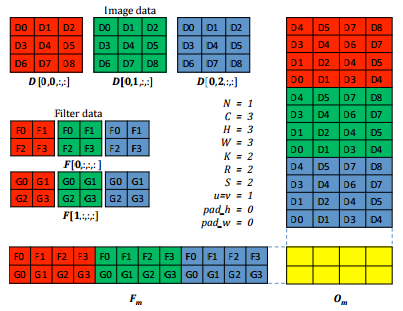
\includegraphics[width=0.6\linewidth]{images/5_convolution}
\caption[]{Schema der Faltung als Matrix-Matrix-Multiplikation (siehe \cite{Chetlur14})}
\label{fig:5_convolution}
\end{figure}

Die Reduktion funktioniert, indem einerseits die verschiedenen Filtermasken ausgerollt werden und andererseits Filtermasken, die zu einer \textit{Feature-Map} gehören hintereinander in einen Zeilenvektor konkateniert werden. Mehrere solcher Zeilenvektoren werden zu einer Matrix $F_m$ zusammengefasst. Außerdem müssen die einzelnen Bildausschnitte, welche mit den Masken gewichtet werden, ebenfalls ausgerollt und jede \textit{Input-Map} untereinander in einen Spaltenvektor konkateniert werden. Jede gültige Stelle der Eingabe wird so zu einer Matrix $I_m$ zusammengefasst. Als Ergebnis erhält man zwei Matrizen die mittels GEMM berechnet werden können. Die Berechnung eines Convolution-Layer wird so durch Formel \ref{eq:vecminibatch2} beschrieben, wobei entsprechend erweiterte Schwellwerte $B$ zur Anwendung kommen.

\begin{equation}
\label{eq:vecminibatch2} 
\phi(F_m I_m + B)
\end{equation}

Um wieder die Struktur der ursprünglichen Eingabe zu erhalten, müssen die resultierenden Zeilenvektoren $O_m$ nochmals entsprechend umorganisiert werden.
Diese Methode lässt sich auch auf \textit{Mini-Batch}-Training erweitert, indem mehrere Trainingsbeispiele analog zum Hidden-Layer spaltenweise konkateniert werden.

Grundsätzlich können Faltungsoperationen performant mittels der schnellen Fourier-Transformation im Frequenzbereich berechnet werden. Für die Anwendung im Bereich CNNs ist diese Methode allerdings nicht unbedingt von Vorteil, da beispielsweise die Filtergröße im Vergleich zur Eingabegröße gerade in den ersten Schichten sehr viel kleiner ist oder die Faltung mit größeren Schrittweiten (\textit{$Stride > 1$}) angewandt wird \cite[vgl.][]{Chetlur14}.

\subsection{Parallelisierung}
Betrachtet man die Verteilung der Rechenressource innerhalb eines CNN, fällt auf, dass 90 \% der Rechenzeit, aber nur 5 \% der Parameter auf die Convolution-Layer entfällt \cite[vgl.][]{Krizhevsky2014}. Daher bietet es sich an, die in \cite{Krizhevsky2014} vorgeschlagenen Strategien zu verwenden und zwar Daten-Parallelisierung in den Convolution-Layern und Modell-Paralleli\-sier\-ung in den Hidden-Layern.

Aus Gründen der Einfachheit und aufgrund der Tatsache, dass der CPU-basierte Prototyp für große Netze ohnehin nicht geeignet ist, wird auf Model-Parallelisierung verzichtet und das gesamte Netzwerk auf Basis der Daten parallelisiert. 
In \textit{ConvNetCPP} basiert die Parallelisierung auf OpenMP und damit auf parallel ausgeführten For-Schleifen. Ein \textit{Mini-Batch} wird somit auf die zur Verfügung stehende Threads aufgeteilt. Die Strategie ist unterteilt in drei Schritte.

\begin{enumerate}
\item Initialisierung \textemdash\space Jeder Thread bekommt eine Kopie der Modellarchitektur, inklusive eigenem Speicher für Gradient und Aktivierungen.

\item Parallelisierung \textemdash\space Der aktuelle \textit{Mini-Batch} wird auf die einzelnen Threads aufgeteilt und die Netzaktivierung (\textit{Forward Pass}) sowie die Gradientenberechnung (Backward Pass) werden lokal ausgeführt.

\item Zusammenführung \textemdash\space Die berechneten Gradienten werden über die Threads gemittelt und die Parameter aktualisiert.
\end{enumerate}


\subsection{Debugging}
\label{ch:debug}
Die Implementierung eines CNN oder eines Convolutional Autoencoder ist sehr fehleranfällig und im Allgemeinen schwierig zu debuggen. Eine sehr nützliche Methode die Richtigkeit der berechneten Gradienten in neuronalen Netzen zu überprüfen ist die Finite-Differenzen-Methode (vgl. z. B. \cite{Bouvrie2006}). Die Approximation zweiter Ordnung an die partiellen Ableitungen liefert eine bessere Genauigkeit und kann mit Formel \ref{eq:finitediff} berechnet werden (vgl. \cite{Bengio2012}).

\begin{equation}
\label{eq:finitediff} 
\frac{\partial J}{\partial w_i}  \approx \frac{J(w_i + \epsilon) - J(w_i - \epsilon)}{2 \epsilon}
\end{equation}

Mittels dieser Methode kann die Richtigkeit der im Convolutional Autoencoder (siehe Kapitel \ref{ch:autoenc}) gemachte Anpassung erfolgreich überprüft werden.
